\documentclass{article}
\usepackage{graphicx}
\usepackage{wrapfig}
\usepackage{subcaption}
\title{Tophat Condor 2 Connection Instructions}
\date{2020-11-13}
\author{Extension of Instructions found in the Condor 2 Manual}
\begin{document}
    \maketitle

    \section{Prerequisites}
    You'll need a modem/router setup with the device running Condor 2
    and the device with Tophat installed on the same LAN network. Either device
    can be connected over WiFi or using an ethernet cable. An internet connection will
    also be needed if the HW VSP3 program has not yet been installed.

    \section{Install HW VSP3}
    HW VSP3 is used to create a virtual serial COM port on the device running Condor 2.
    This COM port will be used by Condor 2 to transmit data to the device with Tophat.
    HW VSP3 can be downloaded from:
    \begin{verbatim}
    http://new.hwg.cz/files/download/sw/version/hw-vsp3s_3-1-2.exe
    \end{verbatim}
    Run the installer and follow the instructions. Choose the standalone installation
    (without Server/Client option).

    \begin{figure}[h!]
        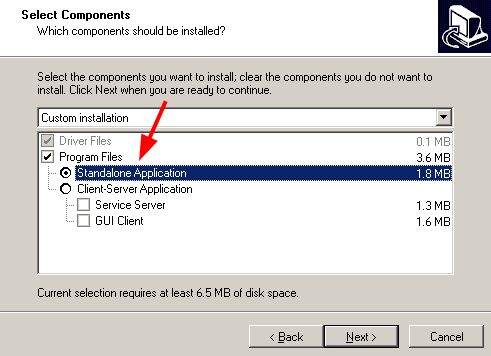
\includegraphics[width=250px]{images/hsvp3.png}
    \end{figure}

    \section{IP Address of Tophat Device}
    Finding the local IP address of the device with Tophat installed can be done a number of ways. In almost
    all cases, you won't need to use the 'PC' method unless you're using a Windows PDA or some other
    PC like device. Hold onto this address once you find it, you'll need it later.\\
        
        \subsection{Mobile/Tablet}
        \begin{wrapfigure}{r}{0.3\linewidth}
            \vspace{-40pt}
            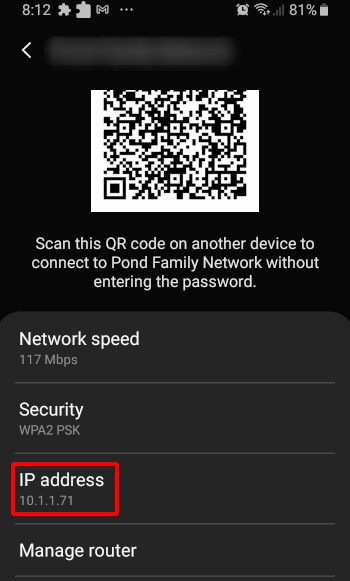
\includegraphics[width=100px]{images/mobile-ip.png}
        \end{wrapfigure}
        The easiest method if the device is a mobile phone or tablet
        is to check the connection settings of the device as the IPv4 address will often be listed there.
        If this method does not work, the 'All' method will work for any device on your LAN network.
        
        \subsection{PC} Open the CMD.exe program and use the `ipconfig' command. The output will be similar
        to the image below. You're looking for the IPv4 address of the device, outlined in red.
        \begin{figure}[h!]
            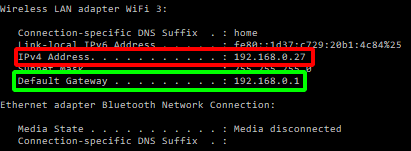
\includegraphics[width=\linewidth]{images/local-ip.png}
        \end{figure}
        
        \subsection{All}
        This method relies on logging into the modem and assumes that you know the login and
        password to your modem. Almost all modems will allow you to log in to their admin portal
        via webpage by going to the address of the modem in your browser. That said, the layout of
        these webpages are often vastly different from each other.
        
        \begin{enumerate}
            \item The address of the modem can be found by running the `ipconfig' command in the CMD program
            and copying the `Default Gateway' address outlined in green in the image above.
            \item Paste the address in the URL bar of your browser and log into the modem using the login and password.
            \item You'll need to find where your modem admin portal lists the connected devices. Mine lists them under
            the `Devices' section, but many other modems will be different.
            \begin{figure}[h!]
                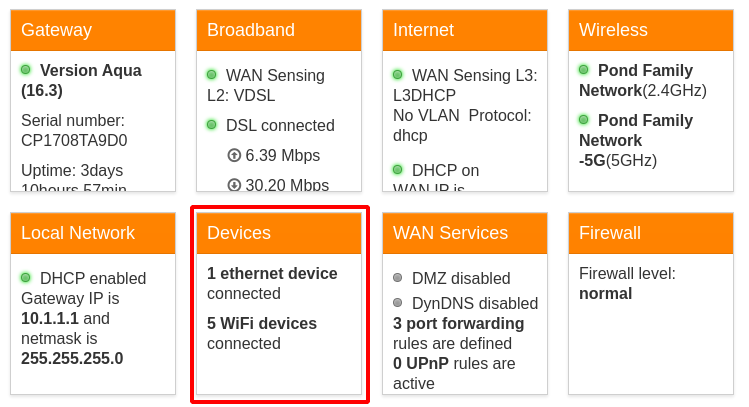
\includegraphics[width=\linewidth]{images/modem-devices.png}
            \end{figure}
            \item Once you've found where the connected devices are displayed, look for name of the device with Tophat
            installed. I have Tophat installed on my phone which is the Galaxy-S8 in this list. The IP Address is what
            we're after.
            \begin{figure}[h!]
                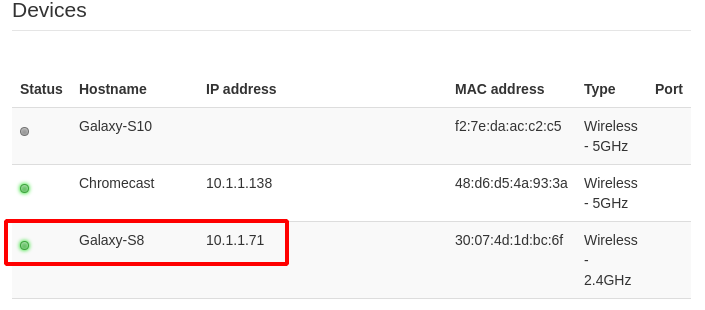
\includegraphics[width=\linewidth]{images/modem-tophat-device.png}
            \end{figure}
        \end{enumerate}

    \section{Configure Tophat}
    Open Tophat on your device and choose `Fly' (Sim doesn't seem to work properly with this setup) navigate to the third
    menu and tap the cog to enter the configuration page (Step 1). Tap `Device' to open the device settings page (Step 2). 
    You will be presented with a list of devices, all of which are disabled by default except for the device's onboard
    senors like GPS, Gyro, etc. Select a free device and tap `Edit' (Step 3). Set the `Port' to TCP Port, this will bring
    up more fields. Set the `TCP Port' to one of the four options and set `Driver' to Condor Soaring Simulator (Step 4).
    Remember the port that you chose, you'll need it later.
    \begin{figure}[h!]
        \centering
        \captionsetup[subfigure]{labelformat=empty}
        \begin{subfigure}[b]{0.24\linewidth}
            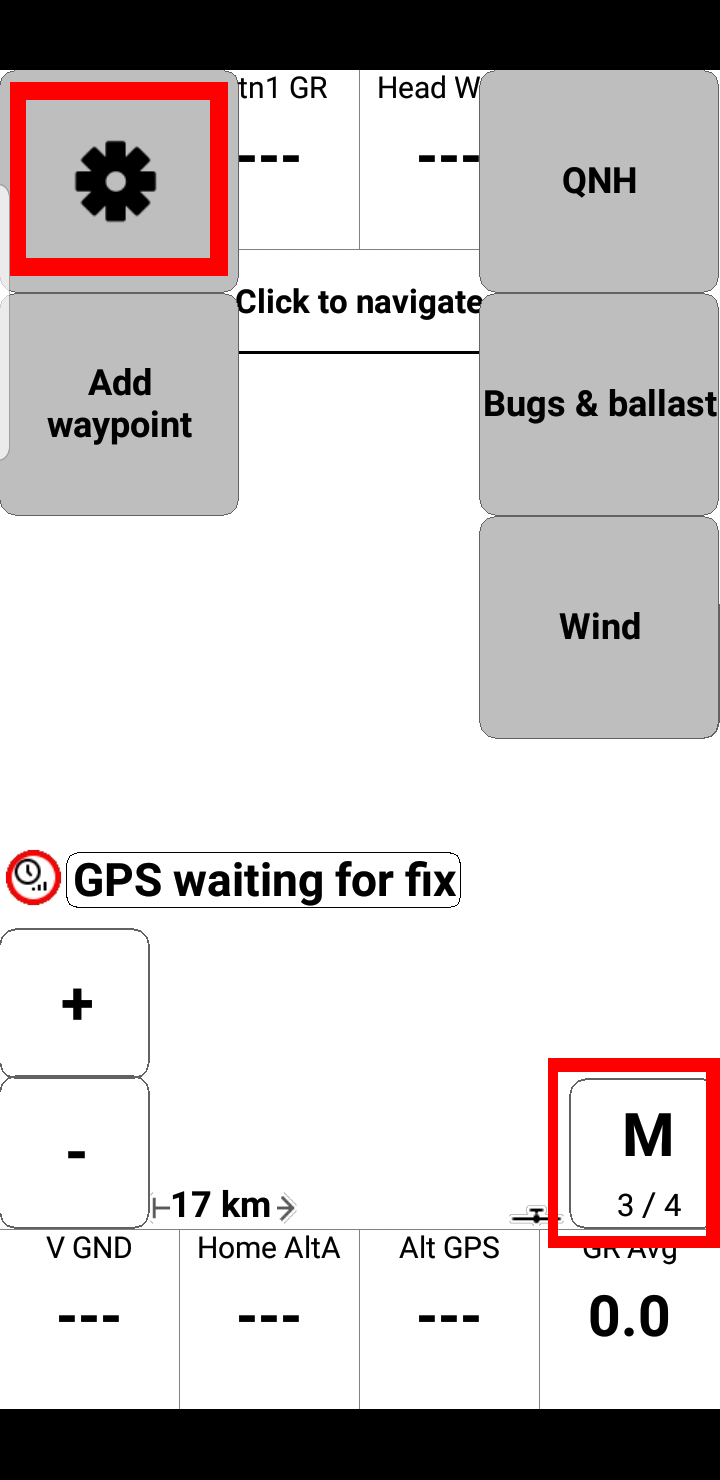
\includegraphics[width=\linewidth]{images/Tophat-1.jpg}
            \caption{Step 1}
        \end{subfigure}
        \begin{subfigure}[b]{0.24\linewidth}
            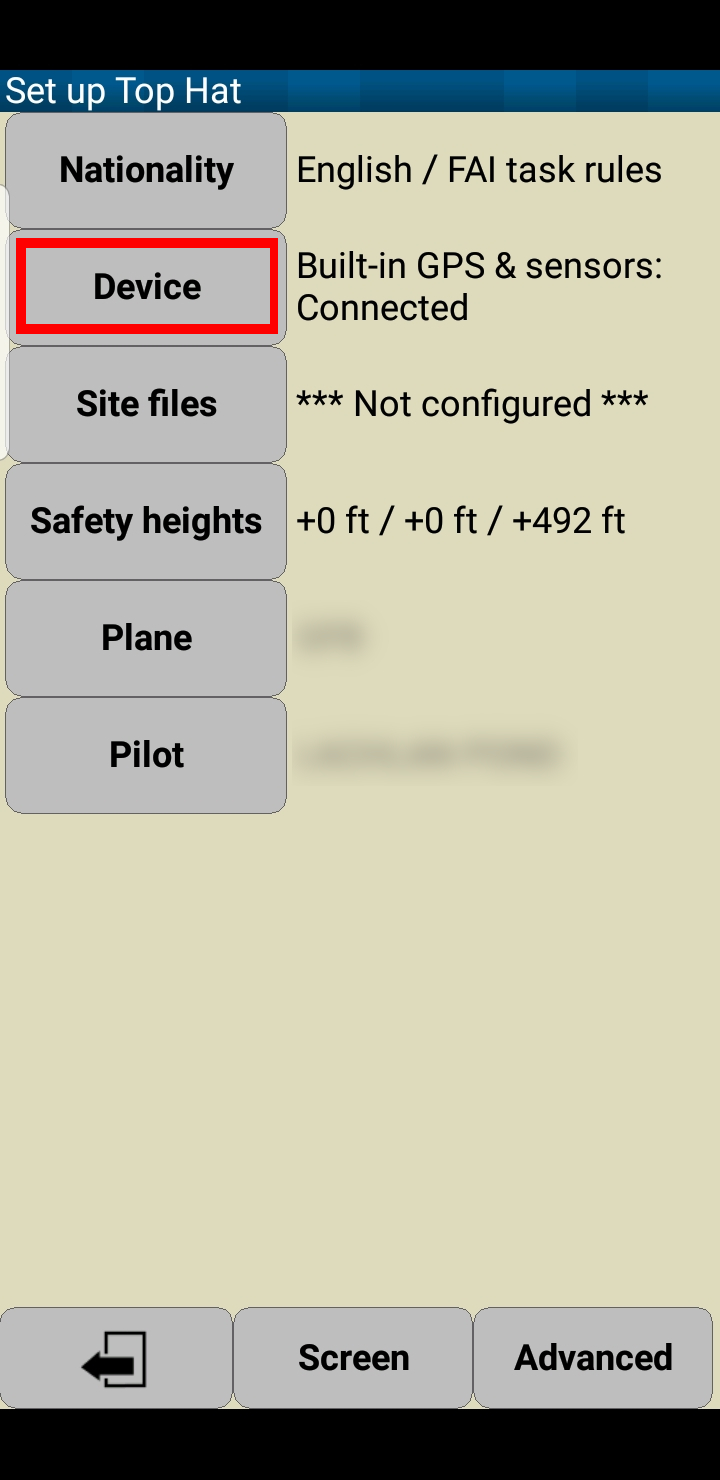
\includegraphics[width=\linewidth]{images/Tophat-2.jpg}
            \caption{Step 2}
        \end{subfigure}
        \begin{subfigure}[b]{0.24\linewidth}
            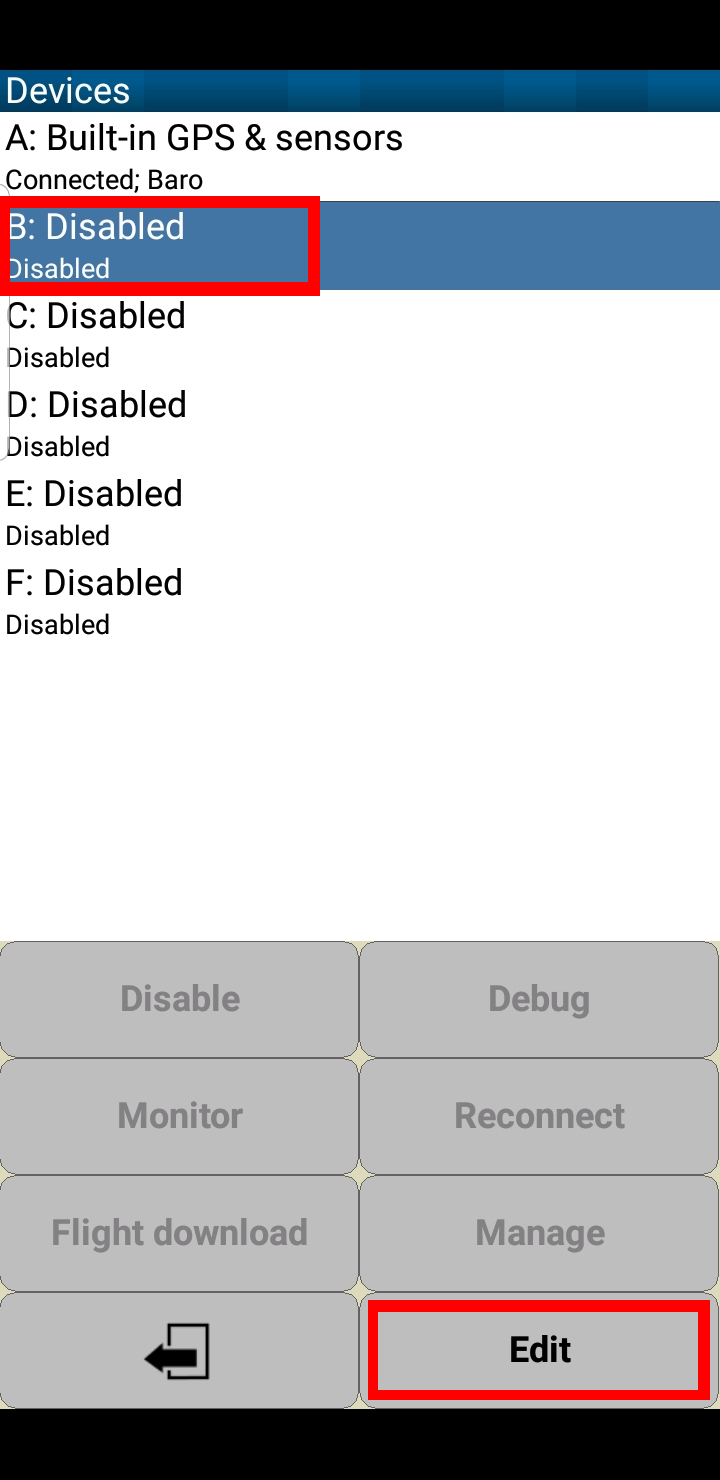
\includegraphics[width=\linewidth]{images/Tophat-3.jpg}
            \caption{Step 3}
        \end{subfigure}
        \begin{subfigure}[b]{0.24\linewidth}
            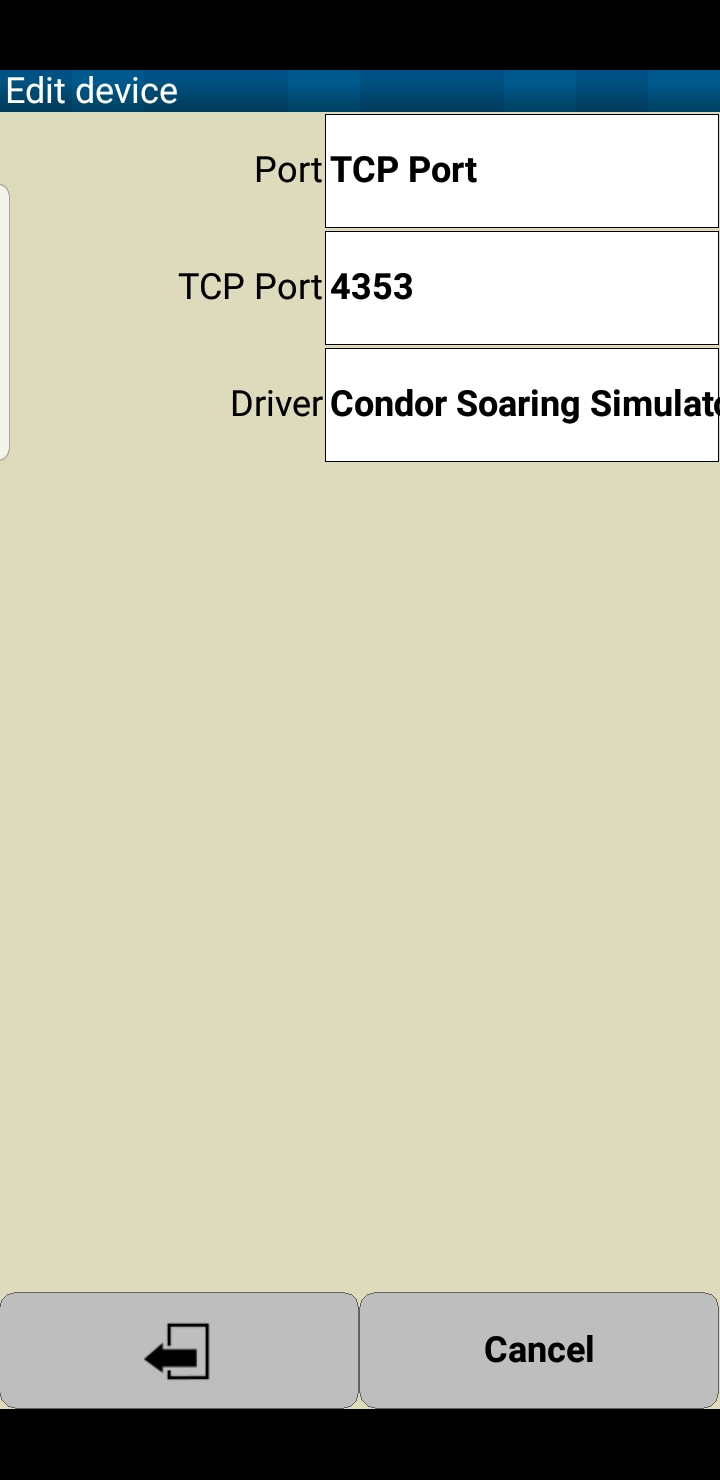
\includegraphics[width=\linewidth]{images/Tophat-4.jpg}
            \caption{Step 4}
        \end{subfigure}
    \end{figure}

    \section{Check Available COM Ports}
    Open Condor 2, navigate to `Settings'\textrightarrow`Options'\textrightarrow`NMEA Output' and check what COM ports appear
    in the dropdown. Any COM ports that appear cannot be used in the next section.

    \section{Setup HW VSP3}

\end{document}